% !TeX root = ../main.tex

\chapter{Experimental Setup}
\label{ch:experimental_setup}

The following chapter describes the experimental setup for the discussion of results in chapter~\ref{ch:discussion}. All classifiers were tested with cross validation using a train - test split ratio of 80\% - 20\%. 5-fold cross validation was only used for the evaluation of the histogram classifier but not for the experiments with the other classifiers since the computational cost for 5-fold cross validation is very high.

\section{Hardware}
\label{sec:hardware}
The training and the evaluation of the classifiers was done on 4 different servers all running Ubuntu. Two of the servers {(Schlichter2 and Schlichter4)} belong to the faculty of applied informatics and the other two are cloud instances. One is an azure virtual compute instance with 8 \gls{cpu} cores and 28 \gls{gb} of \gls{ram} and the other is an Amazon EC2 g2.2xlarge \gls{gpu} instance with a Intel Xeon E5-2670 processor, 15 \gls{gb} of \gls{ram} and a NVIDIA Grid K520 \gls{gpu}. See table \ref{tab:usedHardware} for more details.
\begin{table}[hbt]
	\centering
	\caption{Used hardware for model training and evaluation.}
	\label{tab:usedHardware}
	\begin{tabular}{@{}ccccc@{}}
		\toprule
		\multicolumn{1}{c}{\textbf{}}    & \multicolumn{1}{c}{\textbf{OS}} & \multicolumn{1}{c}{\textbf{CPU}}                    & \multicolumn{1}{c}{\textbf{RAM}} & \multicolumn{1}{c}{\textbf{GPU}}     \\ \midrule
		Schlichter 2 & Ubuntu 12.04              & Intel Core i7-3930K @ 3.20GHz   & 63 GB        & NVIDIA Titan X \\ \midrule
		Schlichter 4 & Ubuntu 14.04              & Intel Xeon E5-2620 @ 2.00GHz    & 28 GB        & -                \\ \midrule
		Azure        & Ubuntu 15.10              & Intel Xeon E5-2673 v3 @ 2.40GHz & 28 GB        & -                \\ \midrule
		Amazon AWS   & Ubuntu 14.04              & Intel Xeon E5-2670              & 15 GB        & NVIDIA K520 \\ \bottomrule
	\end{tabular}
\end{table}

\section{Datasets}
The classifiers are primarily evaluated on two datasets. For the parameter optimization a smaller 8-class subset of the UEC Food-100 dataset is used because the computational cost of training on huge datasets is very high. The 8 classes from the original dataset were selected randomly. The dataset consists of the classes

\begin{enumerate}
	\item Beef
	\item Croissant
	\item Eels
	\item Egg hotchpotch
	\item Hamburger
	\item Pizza
	\item Sashimi
	\item Sauteed burdock
\end{enumerate}
The sampled dataset is very imbalanced with a mean of 134.5 images per class. The class with the lowest number of images contains 108 images and the class with the highest amount of images has more than twice as much images {(233 images)}.

Each feature classifier is then also tested on the full 50-data dataset {(50 classes)}. The color histogram is also tested on the complete UEC Food-100 dataset. The other classifiers are not evaluated on this dataset because evaluating the histogram classifier with a 5-fold cross validation took about 42 hours on the azure cloud virtual machine.

The neural networks are not tested on 50-data or Food-100. The number of images per class of 50-data and Food-100 are not sufficient enough for convolutional neural network training. 50-data only contains 5000 images and Food-100 includes 14,357 images. As a compromise between training time and images per class a special dataset is used. To increase the number of images to 2000 images per class, the intersect between ETHZ Food-101, UPMC Food-101, 50-data and Food-100 is formed and the classes are combined. The false positive rate for the UPMC Food-101 dataset is very high so most of the false positive images were manually removed. This dataset consists of 6 classes with an average of 2004 images per class. A smaller net is also evaluated on a smaller subsampled dataset of the 50-data dataset. This subsampled set contains the classes "Arepas", "Braised pork", "bread", "buns", "chaisu", "chicken rice" and "chocolate".

Table \ref{tab:resultsDatasets} accumulates statistics about the used datasets.

\begin{table}[htb]
	\begin{tabular*}{\columnwidth}{@{\extracolsep{\stretch{1}}}*{6}{c}@{}}
		\toprule
		Name			 & Classes  & Images  	& Null Score  	& Mean \# Images & \gls{std} \# \\ \midrule
		50data			 & 50	 	& 4967	 	& 0.0201 		& 99 				& 2\\
		Food-100	 	 & 100		& 14,357	& 0.0507 		& 144 & 87 \\
		Food-100 8-class & 8 		& 1076		& 0.2165 		& 135 & 41 \\
		Big Intersect	 & 6 		& 12,029 	& 0.1893 		& 2005 & 172 \\
		50data 8-class	 & 8 		& 800	 	& 0.125 		& 100 & 0 \\ \bottomrule
	\end{tabular*}
	\caption{Dataset details used for the results in chapter \ref{ch:discussion}.}
	\label{tab:resultsDatasets}
\end{table}

\section{Data Preprocessing}
For all algorithms every image is loaded by OpenCV and resized so that each image has exactly the same image area while keeping the aspect ratio locked. This is extremely important because otherwise the quality and quantity of features that can be extracted from the images varies based on the image size. This variation greatly affects the accuracy. 

In addition, neural nets require a fixed aspect ratio of the input over all images. The aspect ratio $1\times 1$ was chosen because most images are already very close to that ratio and it is generally a common practice to have this kind of input ratio for neural net inputs. If images have a different aspect ratio, they are cropped around the center. If the aspect ratio is smaller than 0.3 or bigger than 3 the image is skipped because cropping would omit too much of the image. The images are not simply resized since the resulting distortion might decrease accuracy.

For most of the algorithms the image is loaded in gray scale. Exceptions are color histograms and neural nets that take color images as input. Color correction, denoising, or contrast adjustments are not performed because while testing they could not improve accuracy and often led to poorer overall results.

Again, neural networks get the image data a little bit differently. The used framework for neural nets requires the data to be scaled to a $[0,1]$ interval, 32-bit floats and be reshaped to $[\text{number of channels} \times \text{width} \times \text{height}]$. All other models get data scaled as normal 8-bit $[0,255]$ pixel values and shaped as $[\text{width} \times \text{height} \times \text{number of channels}]$.

\subsection*{Data Augmentation}
\label{subsec:dataAugmentation}
\begin{figure}[htb]
	\centering
	\hspace{\fill}%
	\subfloat[Original image]{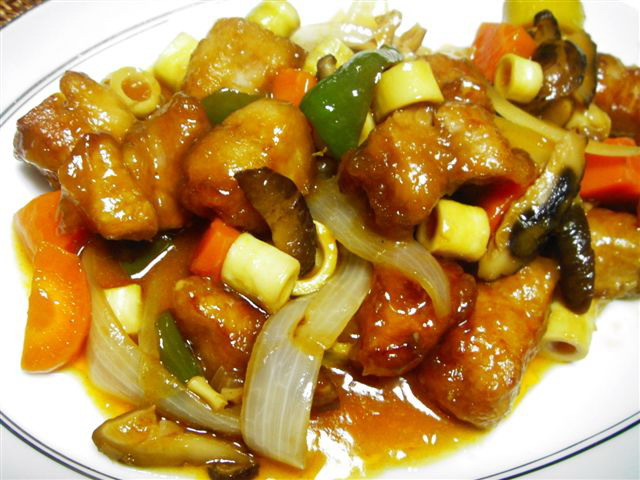
\includegraphics[width=25mm]{data/images/setup/preprocessingDA_original}}
	\hspace{\fill}%
	\subfloat[Increased brightness]{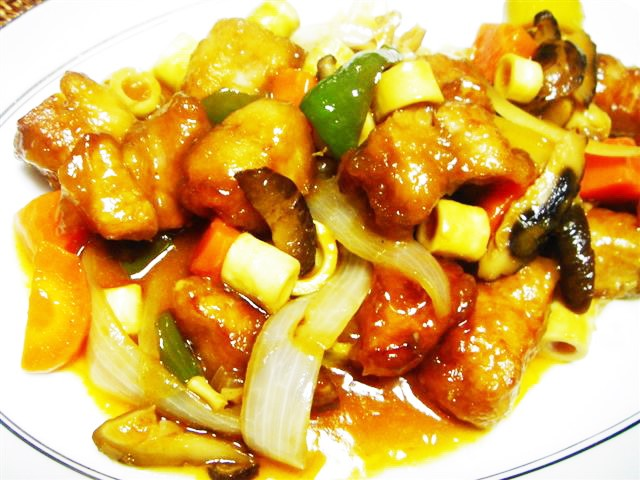
\includegraphics[width=25mm]{data/images/setup/preprocessingDA_brightness}}
	\hspace{\fill}%
	\subfloat[Random cropping]{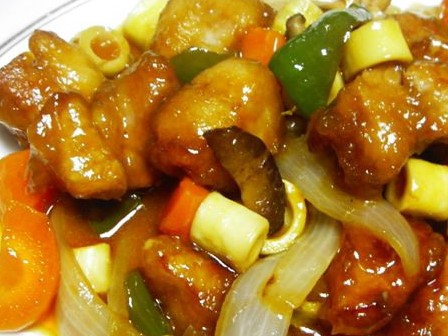
\includegraphics[width=25mm]{data/images/setup/preprocessingDA_crop}}
	\hspace{\fill}%
	\subfloat[20\degree rotation]{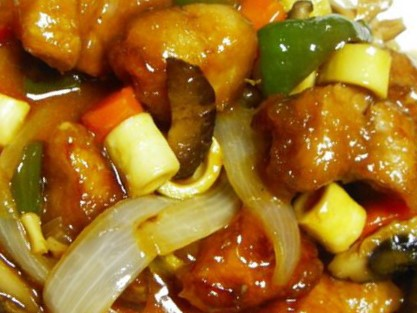
\includegraphics[width=25mm]{data/images/setup/preprocessingDA_rotation}}
	\hspace{\fill}%
	\subfloat[rotation and horizontal flip]{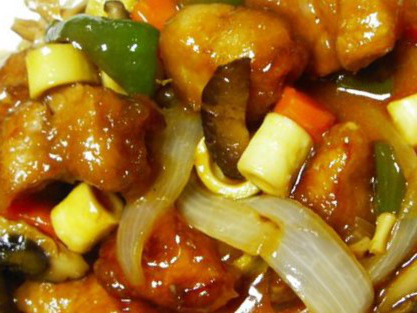
\includegraphics[width=25mm]{data/images/setup/preprocessingDA_rotHorFlip}}
	
	\caption{Examples for label preserving data augmentation.}
	\label{fig:dataAugmentation}
\end{figure}
To reduce overfitting of neural networks data augmentation is performed. Data augmentation is a very common method to artificially increase the size of the dataset by performing label-preserving image altering methods \cite{Dosovitskiy2013, Krizhevsky2012, Christodoulidis2015}. 
	
In this case there are nine operations that can be applied to an image. The maximum number of successive data augmentations on a single image is 4, although, the probability for such operations is linearly decreasing with a probability of 60\% for the first and 15\% for the fourth augmentation.

The first data augmentation category consists of image brightness {(fig. \ref{fig:dataAugmentation}b)} and saturation changes in the \gls{hsv} color space. Brightness and saturation are scaled by an uniform random number in the interval $[0.25,1.75]$. Dosovitskiy et al. proposed to raise these values by a power of up to 4 \cite{Dosovitskiy2013}. However, changing saturation or brightness by 4 increases these values far to much.

The second category contains horizontal- and vertical flipping {(fig. \ref{fig:dataAugmentation}e)} and $[90\degree , 180\degree, 270\degree ]$ rotations.

The last category requires that the images are loaded slightly bigger than the input size for the neural net requires. On the larger images random cropping can be performed {(fig. \ref{fig:dataAugmentation}c)}. Larger image patches also allow "free-rotation" in the interval of $[-30\degree, +30\degree]$ {(fig. \ref{fig:dataAugmentation}d)}. This is done by cropping the image after the rotation so that the area that is cropped away is minimal.


\section{Algorithms Variations}

\subsection{SVMs}
\glspl{svm} are binary classifiers so it's not possible to train all $n$ food classes with $m_i$ images in the $i$-th class directly on them. To solve this problem $n$ One-VS-Rest \gls{svm} are trained {(see section \ref{subsec:svmMulticlass})}. Since there are $n-1$ times more negative samples than positive samples, the negative samples get undersampled so that there is a balance between positive and negative samples. In this case undersampling is done by selecting only $\frac{\mean{m}}{n-1}$ images per class. In contrast to random undersampling, this assures an even distribution of all negative classes in the negative sample space. 

Normally, the data for \glspl{svm} is scale normalized before the training or prediction but for the used \gls{svm} implementation scaling did not affect accuracy. 

\subsection{Color Histograms}
This classification method relies on histograms of pixel color intensities. The classifier computes 3 histograms of an image patch. One for each channel in the \gls{hsv} color space though the color space does not really impact accuracy. \gls{rgb} channels produce the same accuracy rate. 

Histograms are global features which means that the pixel intensity distribution applies to the whole image and any spatial information of the features is lost. To provide some basic spatial information and to increase the size of the feature vector without sacrificing robustness to color changes the image is segmented into multiple image patches. Since there is no reliable component segmentation yet, the image is divided into $n$ rectangular blocks {(instead of component segmentation)}. For each image patch 3 histograms are computed. By concatenating each histogram a feature vector is created.

The classification is then done by a \gls{svm}.

\subsection{Feature Detectors}
The original purpose of feature detectors and descriptors like \gls{sift} {(section \ref{subsec:sift})} or \gls{surf} {(section \ref{subsec:surf})} was to provide reliable matching between different views of the same scene \cite{Lowe2004}. Food classification is different because the task is not to recognize the same object from different angles but to classify similar looking objects into different classes. Therefore, only the keypoint detection and description parts are used and not the additional keypoint matching functionality \gls{sift} and \gls{surf} provide.

The recognition task using \gls{sift}-like classifiers comprises of four steps:
\begin{enumerate}
	\item Keypoint detection
	\item Keypoint description
	\item Feature quantization using a \gls{bow}
	\item Classification using One-VS-Rest \glspl{svm}
\end{enumerate}

\subsubsection*{Keypoint Filtering}
\label{subsub:keypointFiltering}
In the keypoint detection stage, detectors often select false keypoints {(figure \ref{fig:keypointFiltering}a)} because they do not differentiate between relevant points of the food object and edges in the background. Another problem is that the number of extracted keypoints changes, based on the number of image features. A low contrast image has less keypoints than a high contrast image with many edges which leads to problems in the classification stage. So images have either too many or too few keypoints. To solve these problems an additional keypoint selection algorithm is applied after the keypoint detection. It leverages the fact that people who take photos of their food almost always center the food objects in the middle. This makes it possible to weight the keypoint response values $r_i$ with the distance to the center $d_i$ so that a keypoint score can be calculated for all $n$ keypoints. For this score the distance of all keypoints is scaled to the interval $[0, 1]$ with "0" being the closest to the center and "1" being the farthest away. The same is done for the keypoint responses {("0" is a weak keypoint, "1" is a robust keypoint)}. The score $S_i$ is then given as
\begin{equation}
	S_i = 1- (d_i * (1 - r_i)) \quad \forall i, i=1 \dots n
	.
\end{equation}
A high score $S_i \in [0.9, 1]$ means that a keypoint is probably valuable because it is close to the center and therefore describes the object and not the background and it also has a strong response value which means that the point should be robust. The list of keypoints is then sorted by the descending score value. Since the number of extracted keypoints should be the same for all images only the best $m$ keypoints are chosen. Figure \ref{fig:keypointFiltering}b shows the result of this process. In this special case the table surface has a high-contrast texture which \gls{sift} recognizes as keypoints. The filtered version does not contain the irrelevant background keypoints.

For many low-contrast images which lack enough distinctive features, \gls{sift}, \gls{surf} or \gls{fast} provide less than $m$ keypoints. For these cases the algorithm augments existing keypoints. To do this, points are randomly sampled using a Gaussian distribution around the mean of all sampled keypoint positions. The standard deviation equals 0.5 the standard deviation of the keypoint positions. The result of this imputation is shown in figure \ref{fig:keypointFiltering}c.

\begin{figure}[htb]
	\centering
	\hspace{\fill}%
	\subfloat[Unfiltered \gls{sift} keypoints]{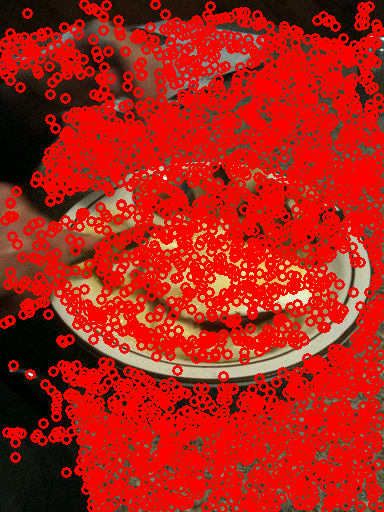
\includegraphics[width=35mm]{data/images/setup/algorithmsSIFT_noFiltering}}
	\hspace{\fill}%
	\subfloat[Filtered \gls{sift} keypoints]{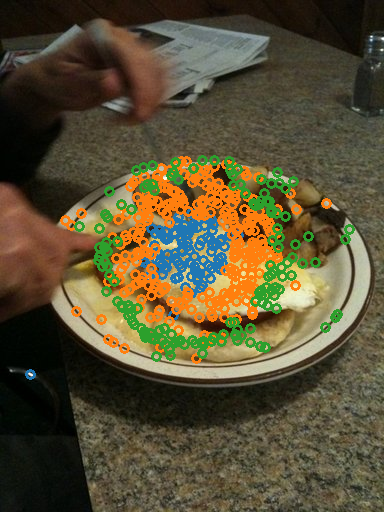
\includegraphics[width=35mm]{data/images/setup/algorithmsSIFT_filtering}}
	\hspace{\fill}%
	\subfloat[\gls{sift} keypoints {(red)} and augmented keypoints {(green)}]{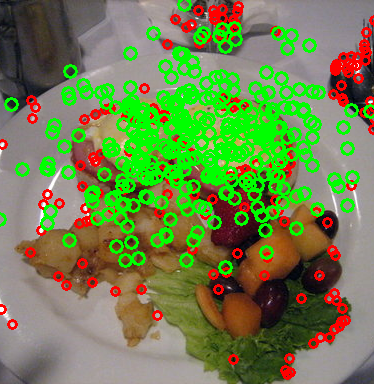
\includegraphics[width=35mm]{data/images/setup/algorithmsSIFT_augmention}}
	\hspace{\fill}%
	\caption{\gls{sift} keypoint filtering and imputation with $m=600$ keypoints.}
	\label{fig:keypointFiltering}
\end{figure}


\subsection{Neural networks}
\label{subsec:setupNN}

\subsubsection*{Learning Rate and Momentum}
Learning rate and momentum are important hyperparameters. Especially with the learning rate and momentum, there are problems if they are fixed. By using a low learning rate the network learns very quickly but may not learn a good model if it oversteps the global minima. If the learning rate is two low it takes many epochs to train the network and it might even get stuck on a local minima.

By adjusting the values dynamically most of these problems can be solved. Learning rate and momentum are adjusted in the same way although they have both different starting values. For the fist 50 epochs both values are linearly decreased to $\sfrac{1}{5}$ of the start value. For the next 50 epochs they retain this value and after the 100th epoch momentum and learning rate are again linearly decreased until they reach $\sfrac{1}{500}$ of the value after the 100th epoch.

\subsubsection*{Early Stopping}
Many complex neural networks suffer from overfitting if trained to long. To prevent overfitting on a good network, the training is stopped and restored if the loss on the validation set has not improved for 100 consecutive epochs.

\subsection{Size Estimation}
Portion size estimation using images is extremely difficult. To get accurate measurements of weight an algorithm has to calculate volume and has to correctly classify an image to determine the density of the food. Volume estimation is difficult even for state of the art neural networks \cite{Meyers2015} so the developed algorithm will instead focus on area estimation of meal plates and meal parts.

\subsubsection*{Meal Size Estimation}
\begin{figure}
	\centering
	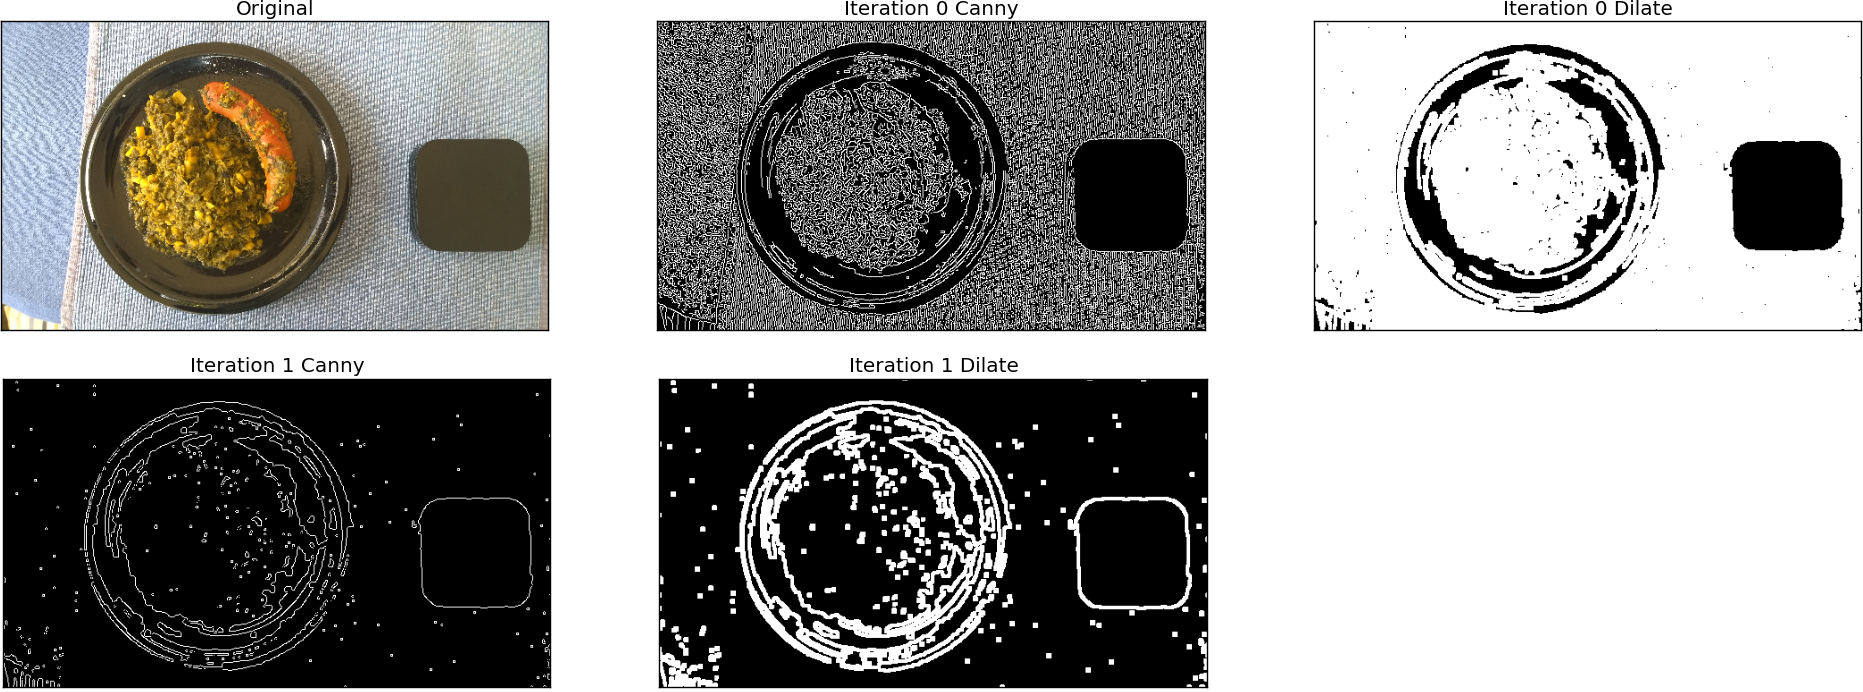
\includegraphics[width=\linewidth]{figures/setup_edgeDetection}		
	\caption{Edge detection process on difficult image. From left to right: a: Original image, b: Image after first Canny operation, c: Canny image after dilation, d: Canny applied on dilated image, e: canny again to close gaps in the plate edge.}
	\label{fig:edgeDetection}
\end{figure}
The basic idea behind the algorithm is based on arbitrary markers of known sizes besides the meal plate. When the size of the marker and the meal in the image is known, the real world meal area can be approximated. Therefore, the goal is to find the plate and the marker.

The first step to reach this goal is to find objects. This is done by applying Canny edge detection \cite{Canny1986}, an extremely popular edge detection algorithm on the image. Sometimes the table surface itself is textured like in figure \ref{fig:edgeDetection}a. In this case the output of the edge operation is not very useful since it has to much noise {(figure \ref{fig:edgeDetection}b)}. To solve this problem the image is dilated which reduces the noise {(figure \ref{fig:edgeDetection}c)} but also blurs edges so canny and dilation are applied again which leads to a clean edge image. This process can also be applied on images with no table texture without reducing the performance in the following object detection step.

In the next step the algorithm searches for the meal and marker regions by iterating over the image objects. This iteration is done by searching for the largest remaining contour in the image and then deleting this contour. If the edge preprocessing was perfect there are only two contours remaining. The marker and the meal. If the marker was not yet found the current image region is added to the list of potential meal regions. If the marker was found and there are potential meal objects the iteration is finished and the size of the meal is estimated based on the size of the marker in the image. The marker can be anything rectangular although a chessboard pattern is more reliable. The chessboard is recognized by a camera calibration algorithm from OpenCV. In case of custom markers the user has to take a closeup or cropped image of the marker and input the size of the custom marker. By using SIFT keypoints the learned marker is matched against potential image regions and if enough matches are found and the ratio between good matches and bad matches is greater than 0.45 the image region is marked as the marker region and the size is calculated by fitting a bounding rectangle around all SIFT keypoints which is shown in figure \ref{fig:markerMatching}.

\begin{figure}
	\centering
	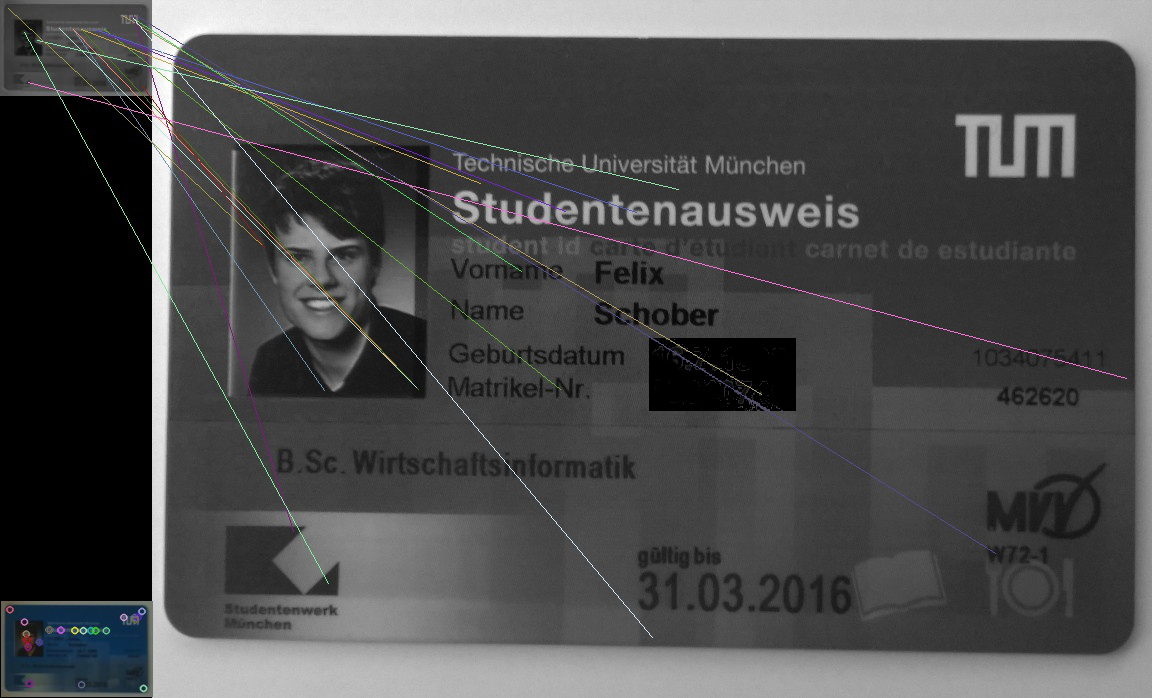
\includegraphics[scale=0.2]{data/images/results/segmentation/resultsMarker_1_matches}		
	\caption{Example of custom marker matching. The figure shows the matching of a learned marker {(top left)} and the matchings between the marker and an image region. Detected keypoints for the bounding rectangle are shown in the bottom left.}
	\label{fig:markerMatching}
\end{figure}

\subsubsection*{Meal Part Size Estimation}
For one-component food items this approach works really well but as soon as a plate contains different kinds of food, this approach becomes inaccurate because the size is measured for the whole plate and not for the components.

This is solved by color filtering the image. To get color filters the 10 most common colors in the meal are calculated by a modified median cut algorithm by Bloomberg \cite{Bloomberg2008}. The image is then converted into the \gls{hsv} color space and filtered against each of the most common colors which creates an image mask that is used to cut out the meal regions. Figure \ref{fig:colorMasks} shows an example of two color masks. Regions under a certain threshold are discarded. The same marker-principle is then applied and the size of the image parts is calculated.

\begin{figure}[htb]
	\centering
	\hspace{\fill}%
	\subfloat[4/4 items detected]{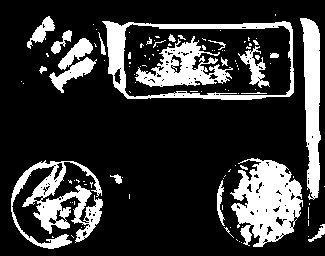
\includegraphics[width=50mm]{data/images/results/segmentation/resultsMask_1}}
	\hspace{\fill}%
	\subfloat[3/3 items detected]{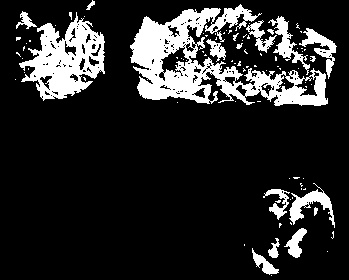
\includegraphics[width=50mm]{data/images/results/segmentation/resultsMask_2}}
	\hspace{\fill}%
	\caption{Color masks after calculation of dominant color palette.}
	\label{fig:colorMasks}
\end{figure}